\documentclass[12pt, a4paper]{article}
\usepackage[utf8]{inputenc}
\usepackage{appendix}
\usepackage{graphicx}
\usepackage{enumerate}
\usepackage{subfig}
\usepackage{float}
\usepackage{indentfirst}
\usepackage{amsmath}
\usepackage{amsfonts}
\usepackage{geometry}   %设置页边距的宏包
\usepackage{titlesec}   %设置页眉页脚的宏包
\usepackage{enumitem}
\usepackage{booktabs}
\usepackage{subfigure}
\usepackage[section]{placeins}
\geometry{left=2.54cm,right=2.54cm,top=2.54cm,bottom=2.54cm}


\begin{document}

\pagestyle{plain}

\begin{titlepage}

	\begin{center}	
	% Title

	\vspace{10ex}

	\hrule

	\vspace{2ex}

	\textbf{\Large{UM-SJTU} \Large{J}\large{oint} \Large{I}\large{nstitute} \\
	\Large{P}\large{HYSICS} \Large{L}\large{ABORATORY} \\
	\large{(}\Large{V}\large{P241)}}\\
	
	\vspace{2ex}

	\hrule
	
	\vspace{25ex}
	
	\Large{L}\large{ABORATORY} \Large{R}\large{EPORT}

	\vspace{6ex}

	\large{E}\normalsize{XERCISE 5}

	\vspace{4ex}

	% lab name here
	\large RC, RL, \normalsize AND \large RLC C\normalsize IRCUITS

	\vspace{4ex}

	% group member here
	\begin{center}
		\begin{tabular}{lll}
		Name: Zhang Jiache & ID: 520370910044 & Group: 9
		\end{tabular}
	\end{center}

	% Bottom of the page
	{\large Date: \today}
	
	\end{center}
	
\end{titlepage}

\newpage

\section{Introduction}
The objective of this lab is to test the physics of alternating-current 
circuits, in particular the charging and discharging process of capacitors, the phenomenon
of electromagnetic induction in inductive elements, and other dynamic processes in 
\textit{RC}, \textit{RL}, and \textit{RLC} series circuits. Also we learn and use the methods for measuring the 
amplitude-frequency and the phase-frequency characteristics of \textit{RC}, \textit{RL}, and \textit{RLC} series 
circuits. We can also derive the resonance frequency of a \textit{RLC} circuit as well as the quality 
factor of the circuit from the amplitude-frequency curve.

\section{Theoretical Background}
\subsection{Transient Processes in RC, RL, RLC Series Circuits}
\subsubsection{RC Series Circuits}
\begin{figure}[H]
	\centering
	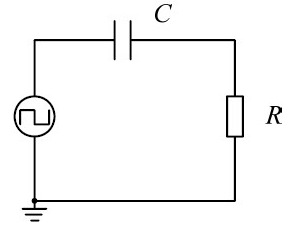
\includegraphics[scale=0.6]{fig1.jpg}
	\caption{RC series circuit.}
\end{figure}
Figure 1 is the simplist example of a \textit{RC} circuit. The charging or discharging process of a \textit{RC} 
circuit is a transient process. When we use a square-wave signal as the voltage with a max voltage of $\mathcal{E}$.
Then the equation for the charging process is:
$$U_C=\mathcal{E}(1-e^{-\frac{t}{RC}})$$
$$U_R=\mathcal{E}e^{-\frac{t}{RC}} $$
For the discharging process:
$$ U_C=\mathcal{E}e^{-\frac{t}{RC}} $$
$$ U_R=-\mathcal{E}e^{-\frac{t}{RC}} $$

where the magnitudes of both $ U_C $ and $ U_R $ decrease exponentially with time. The curves can be draws as:
\begin{figure}[H]
	\centering
	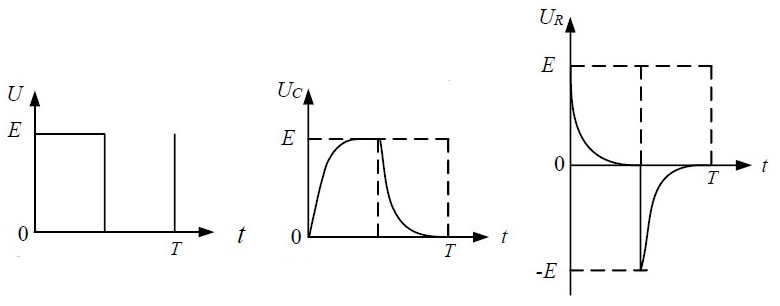
\includegraphics[scale=0.6]{fig2.jpg}
	\caption{Charging/discharging curves for a RC series circuit.}
\end{figure}
We can also derive that $RC = \tau$ and it is called the time constant of the circuit. 
So that the half-time period is:
$$ T_{1/2} = \tau\ln2\approx0.693\tau $$

\subsubsection{RL Series Circuit}
The equations for a RL Series is almost the same, and the equations for charging process can be derived as:
$$U_L=\mathcal{E}(1-e^{-\frac{tR}{L}})$$
$$U_R=\mathcal{E}e^{-\frac{tR}{L}} $$
For discharging process:
$$ U_L=\mathcal{E}e^{-\frac{tR}{L}} $$
$$ U_R=-\mathcal{E}e^{-\frac{tR}{L}} $$
We can also have the time constant and half-time period:
$$\tau  = \frac{L}{R}\quad\text{and}\quad T_{1/2} = \frac{L}{R}\ln2 $$

\subsubsection{RLC Series Circuit}
When a power source is suddenly added to a RLC circuit, We can derieve the loop equation with KVL:
$$\dfrac{d^2U_C}{dt^2}+2\beta\dfrac{dU_C}{dt}+\omega_0^2U_C=\omega_0^2\mathcal{E}$$
Where $\beta = \frac{R}{2L}$ and $\omega_0 = \frac{1}{\sqrt{LC}}$.
By adding initial conditions:
$$U_C(t=0)=0 \text{ and } \left.\dfrac{dU_C}{dt}\right|_{t=0}=0$$
We can split it into 3 different situations and the each has a solution equation:
\begin{enumerate}
	\item
	If $ \beta^2-\omega_0^2<0 $ (weak damping), the system is in the underdamped regime and the solution to the initial value problem is of the form
	$$ U_C=\mathcal{E}-\mathcal{E}e^{-\beta t}\left( cos\omega t+\dfrac{\beta}{\omega}sin\omega t \right) $$
	where $ \omega=\sqrt{\omega_0^2-\beta^2} $
	\item
	If $ \beta^2-\omega_0^2>0 $ (strong damping), the system is in the overdamped regime with the	solution of the form
	$$  U_C=\mathcal{E}-\dfrac{\mathcal{E}}{2\gamma}e^{-\beta t}[(\beta+\gamma)e^{\gamma t}-(\beta-\gamma)e^{-\gamma t}]  $$
	where $ \gamma=\sqrt{\beta^2-\omega_0^2} $
	\item
	If $ \beta^2-\omega_0^2=0 $ the system is said to be critically damped, and
    $$ U_C=\mathcal{E}-\mathcal{E}(1+\beta t)e^{-\beta t} $$
\end{enumerate}
When the source is suddenly removed, we can derieve a similar equation. The overall curve for this process is shown in Figure 3.
\begin{figure}[H]
	\centering
	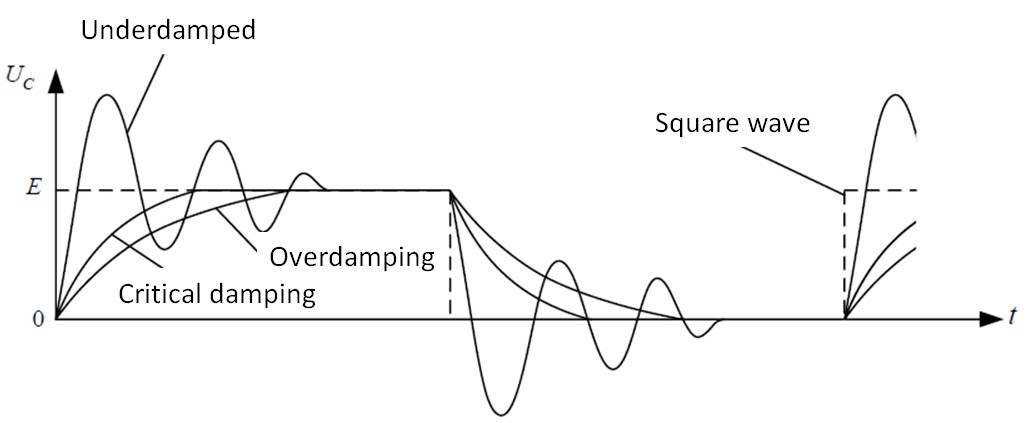
\includegraphics[scale=0.5]{fig3.jpg}
	\caption{Three different regimes of transient processes in a RLC series circuit}
\end{figure}

\subsection{RC, RL Steady-State Circuits}
When a sinusoidal alternating input voltage is provided to a RC or RL series circuit, 
the amplitude and the phase of the voltage across the capacitor and the resistor will 
change with the frequency of the input voltage. Then the amplitude vs. frequency 
relation and the phase vs. frequency relation can be obtained by measuring the voltage 
across the elements in the circuit for different input signal frequencies.
$$ \varphi=tan^{-1}\left(\dfrac{U_L}{U_R}\right)=tan^{-1}\left(\dfrac{\omega L}{R}\right),\qquad \varphi=tan^{-1}\left(-\dfrac{U_C}{U_R}\right)=tan^{-1}\left(-\dfrac{1}{\omega RC}\right) $$
\subsection{RLC Resonant Circuit}
\subsubsection{RLC Series Circuit}
\begin{figure}[H]
	\centering
	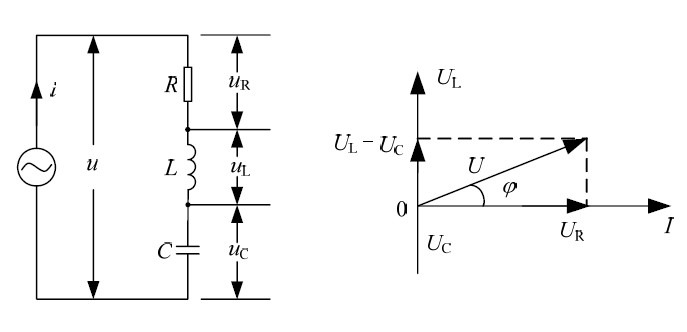
\includegraphics[scale=0.5]{fig4.jpg}
	\caption{RLC series circuit.}
\end{figure}
Above is a generic RLC circuit. The voltage ampitute can be derived as:
$$U=\sqrt{U_R^2+(U_L-U_C)^2} \text{ or } U=I\sqrt{R^2+\left(\omega L-\dfrac{1}{\omega C}\right)^2}$$
And the total impedance is:
$$Z=\sqrt{R^2+\left(\omega L-\dfrac{1}{\omega C}\right)^2}$$
With the phase difference between the current and the voltage in the circuit:
$$\varphi=tan^{-1}\left(\dfrac{U_L-U_C}{U_R}\right)=tan^{-1}\left(\dfrac{\omega L-\frac{1}{\omega C}}{R}\right)$$

\subsubsection{Resonance}
When the current of a RLC circuit reaches its maximum, $ I_m = U/R $, the circuit is said to be at resonance. The frequency
$$ f_0=\dfrac{\omega_0}{2\pi}=\dfrac{1}{2\pi\sqrt{LC}} $$
at which the resonance phenomenon occurs, is called the resonance frequency.

\subsubsection{Quality Factor in Resonant Circuits}
For a circuit driven at the resonance frequency, the ratio of $ U_L $ (or $ U_C $) to U is called the quality factor Q of a resonant circuit
$$ Q=\dfrac{U_L}{U}=\dfrac{\omega_0 L}{R}\text{  or  } Q=\dfrac{U_C}{U}=\dfrac{1}{\omega_0RC} $$

Or it can also be derieve as:
$$ Q=\dfrac{f_0}{f_2-f_1} $$
where $ f_1 $ and $ f_2 $ are two frequencies such that $ I(f_1) = I(f_2) = I_m/\sqrt{2} $.

\section{Experimental setup and Measurement procedure}
\subsection{Apparatus}
The measurement setup consists of the following main elements: a signal generator, 
an oscilloscope, a digital multimeter, a wiring board, a fixed resistor 
$ 100\Omega (2 W) $, a variable resistor $ 2 k\Omega(2 W) $, two capacitors 
$ 0.47 \mu F $ and $ 0.1 \mu F $, as well as two inductors (10 mH and 33 mH).
\subsection{Measurement Procedure}
\subsubsection{RC, RL Series Circuit}
\begin{enumerate}
	\item 
	Assemble a circuit with the fixed-resistance 100 resistor and a capacitor/inductor. 
	Adjust the output frequency of the square-wave signal and observe the change of 
	the waveform when the time constant is smaller or greater than the half-period of 
	the square wave.
	\item 
	Adjust display parameters of the oscilloscope and measure $ T_{1/2} $ for the 
	studied circuits. Then, calculate the time constant and compare it with the 
	theoretical value.
\end{enumerate}
\subsubsection{RLC Series Circuit}
\begin{enumerate}
	\item Assemble a RLC series circuit with the variable resistor, a capacitor and a inductor.
	Observe the waveform of the capacitor voltage in the underdamped, critically damped, and
	overdamped regimes.
	\item Adjust the variable resistor to the critically damped regime. Then measure the half-time period $T_{1/2}$,
	 the time constant $\tau$ and compare them with the theoretical value.
\end{enumerate}
\subsubsection{RLC Resonant Circuit}
Apply a sinusoidal input voltage $ U_i $ to the RLC series circuit, change the 
frequency, then observe the change of the voltage $ U_R $ for a fixed resistor R, 
as well as the phase difference between $ U_R $ and $ U_i $. Measure how $ U_R $ 
changes with $ U_i $ and calculate the phase difference. Plot the graphs 
$ f/f_0 $ vs. $ I/I_m $ and $ f/f_0 $ vs.$ \phi $. Estimate the resonance 
frequency and calculate the quality factor $ Q $.

\section{Results}
\subsubsection{RC, RL Series Circuit}
The measurement data of RC series circuit is shown in the table below:
\begin{table}[H]
	\begin{center}
	\begin{tabular}{|c|c|}
	\hline
	$R$ [$\Omega$] $\pm$ 0.01 [$\Omega$]	&	99.94	\\
	\hline
	$f$ [$Hz$] $\pm$ 0.001 [$Hz$]	&	1000	\\
	\hline
	$\varepsilon$ [$Vpp$] $\pm$ 0.001 [$Vpp$]	&	4.000	\\
	\hline
	$C$ [$nF$] $\pm$ 0.01 [$nF$]	&	99.88	\\
	\hline
	$T_{1/2}$ [$\mu s$] $\pm$ 0.01 [$\mu s$]	&	10.40	\\
	\hline
	\end{tabular}
	\caption{$T_{1/2}$ measurement data for a RC series circuit.}
	\label{tab-1}
	\end{center}
\end{table}
Then we can have:
$$\tau_{theorem} = RC = 9.932\pm0.0014\mu s$$ %%Missing for now.
Compared with the experiment data:
$$\tau_{experiment} = \frac{T_{1/2}}{\ln2} = 15.004\pm0.0014\mu s$$ %%Missing for now.
The image printed in the experiment is:
\begin{figure}[H]
	\centering
	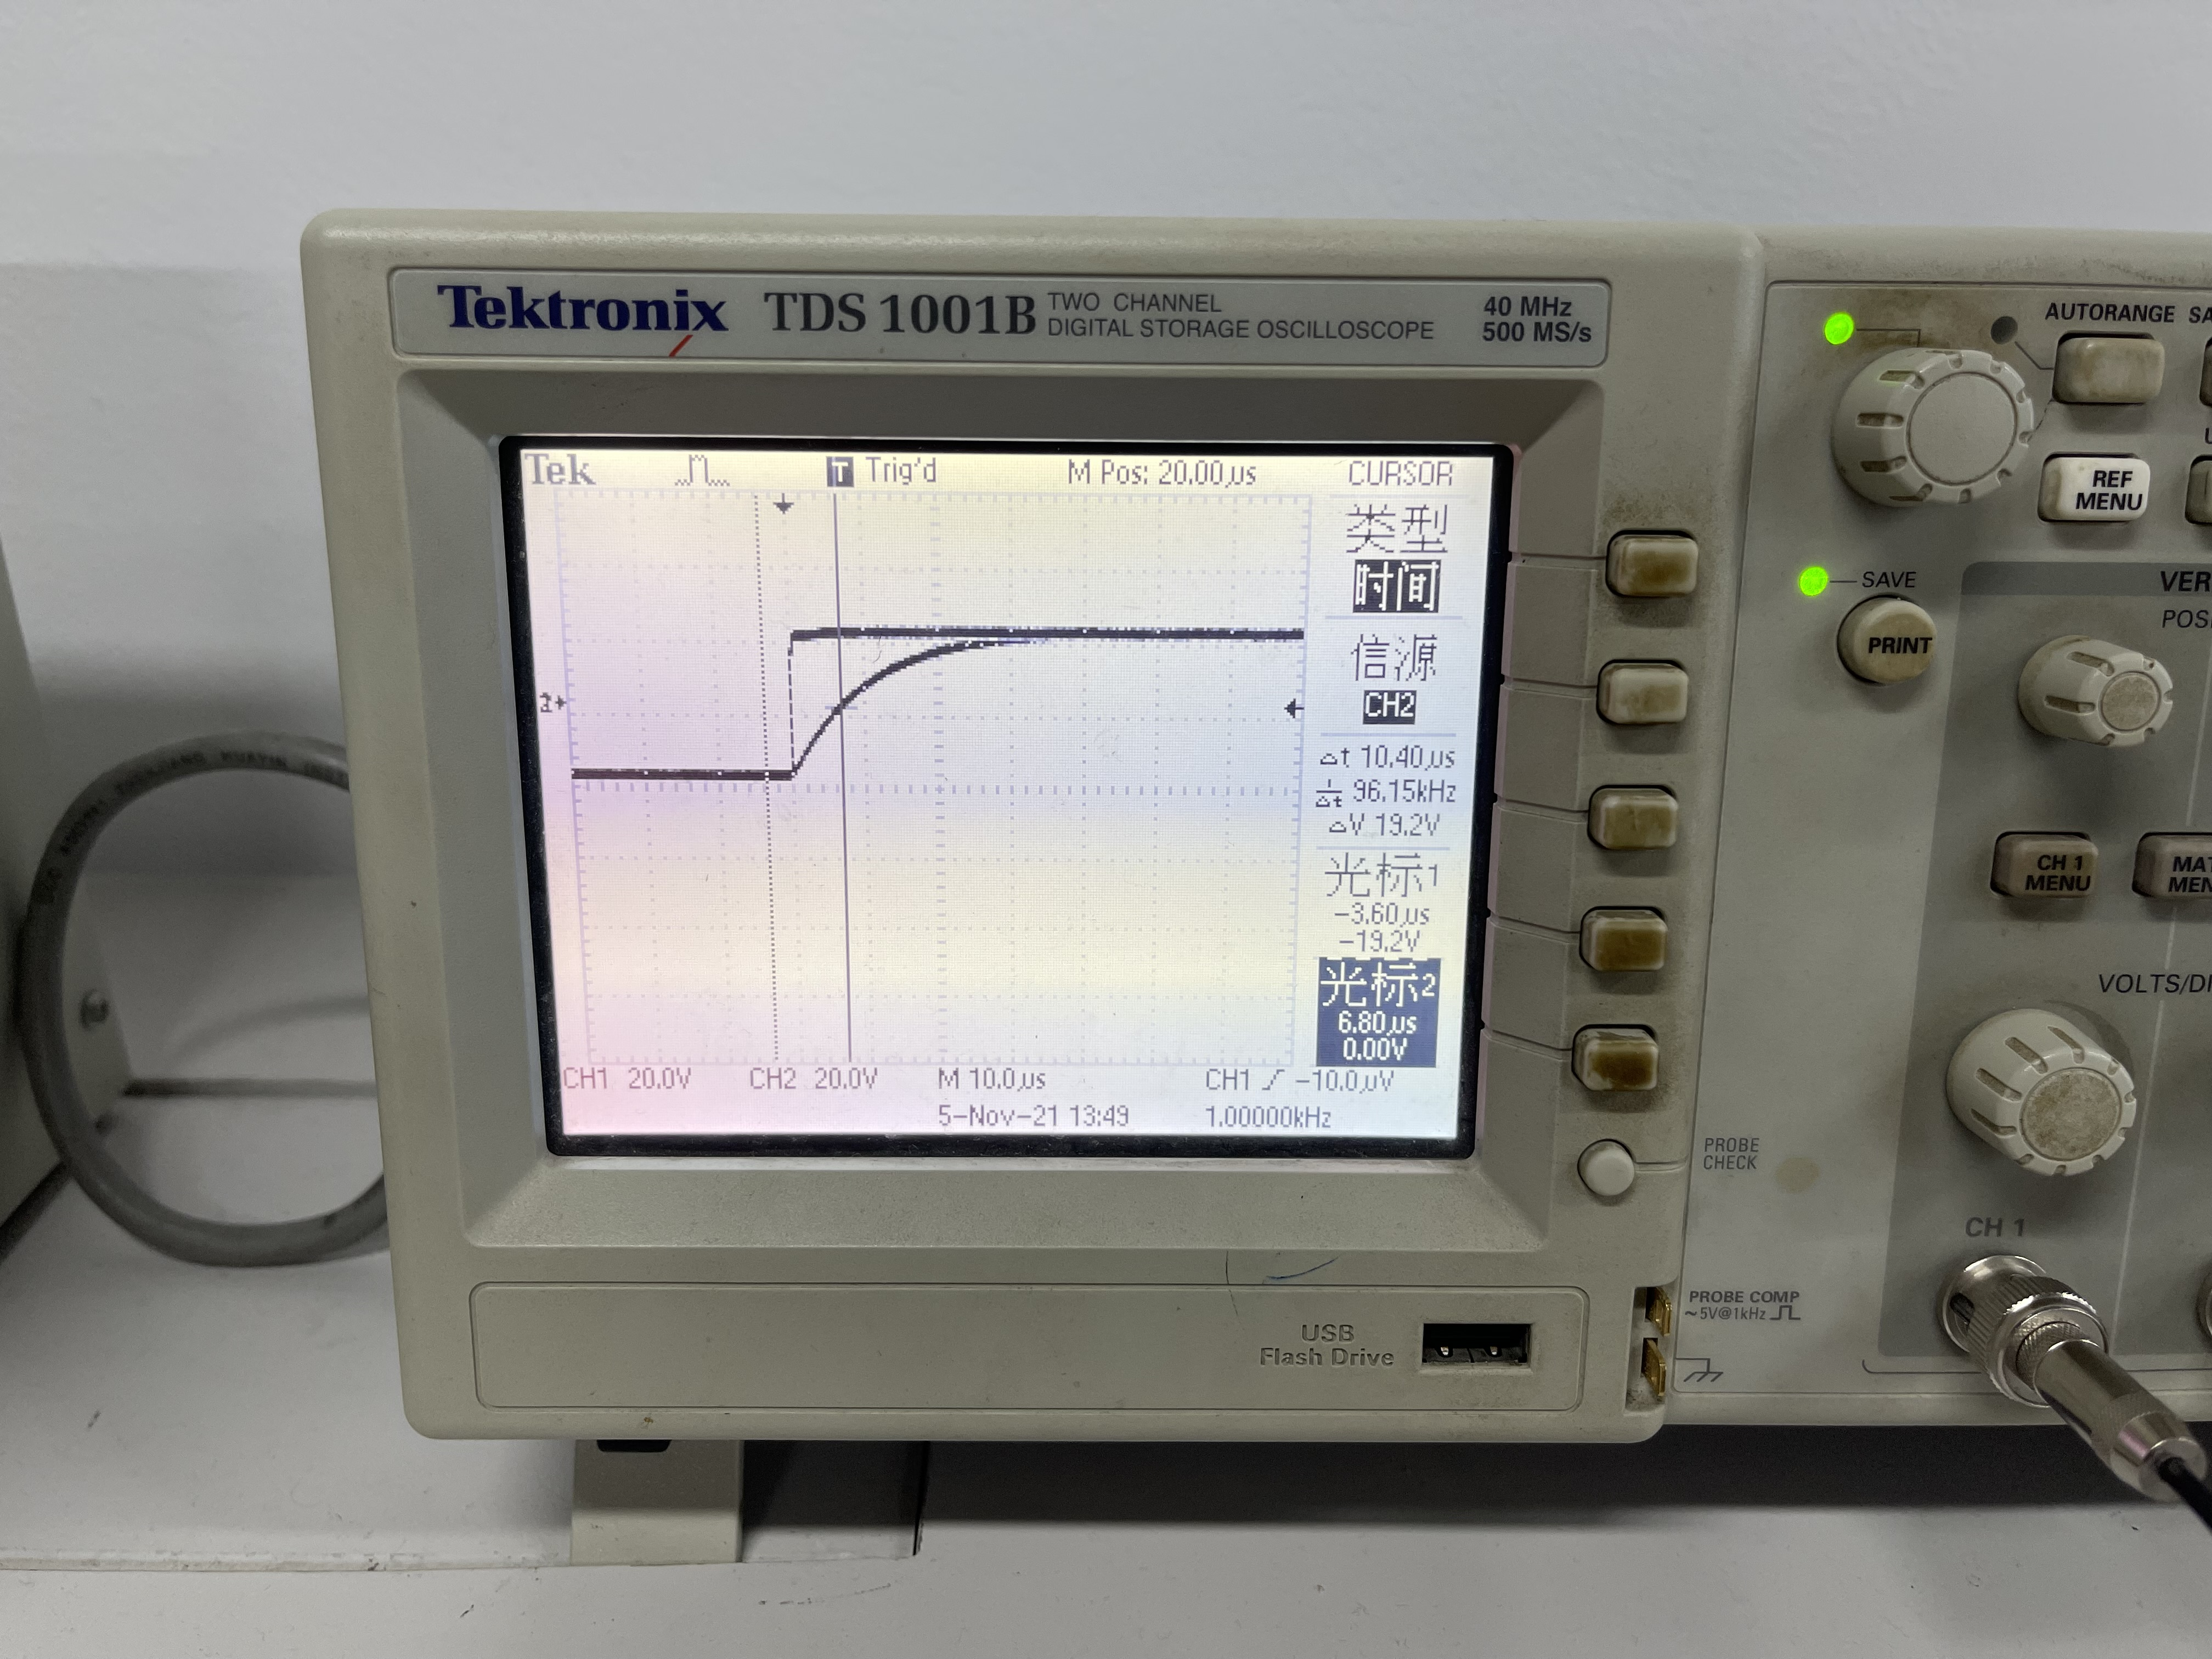
\includegraphics[scale=0.06]{IMG_1829.JPG}
	\caption{RC circuit measurement image}
\end{figure}

The measurement data of RL series circuit is shown in the table below:
\begin{table}[H]
	\begin{center}
	\begin{tabular}{|c|c|}
	\hline
	$R$ [$\Omega$] $\pm$ 0.01 [$\Omega$]	&	99.94	\\
	\hline
	$f$ [$Hz$] $\pm$ 0.001 [$Hz$]	&	1000	\\
	\hline
	$\varepsilon$ [$Vpp$] $\pm$ 0.001 [$Vpp$]	&	4.000	\\
	\hline
	$L$ [$H$] $\pm$ 0 [$H$]	&	0.01	\\
	\hline
	$T_{1/2}$ [$\mu s$] $\pm$ 0.01 [$\mu s$]	&	68.00	\\
	\hline
	\end{tabular}
	\caption{$T_{1/2}$ measurement data for a RL series circuit.}
	\label{tab-2}
	\end{center}
\end{table}
Then we can have:
$$\tau_{theorem} = \frac{L}{R} = 100.06\pm0.014\mu s$$

Compared with the experiment data:
$$\tau_{experiment} = \frac{T_{1/2}}{\ln2} = 98.10\pm0.01\mu s$$
The image printed in the experiment is:
\begin{figure}[H]
	\centering
	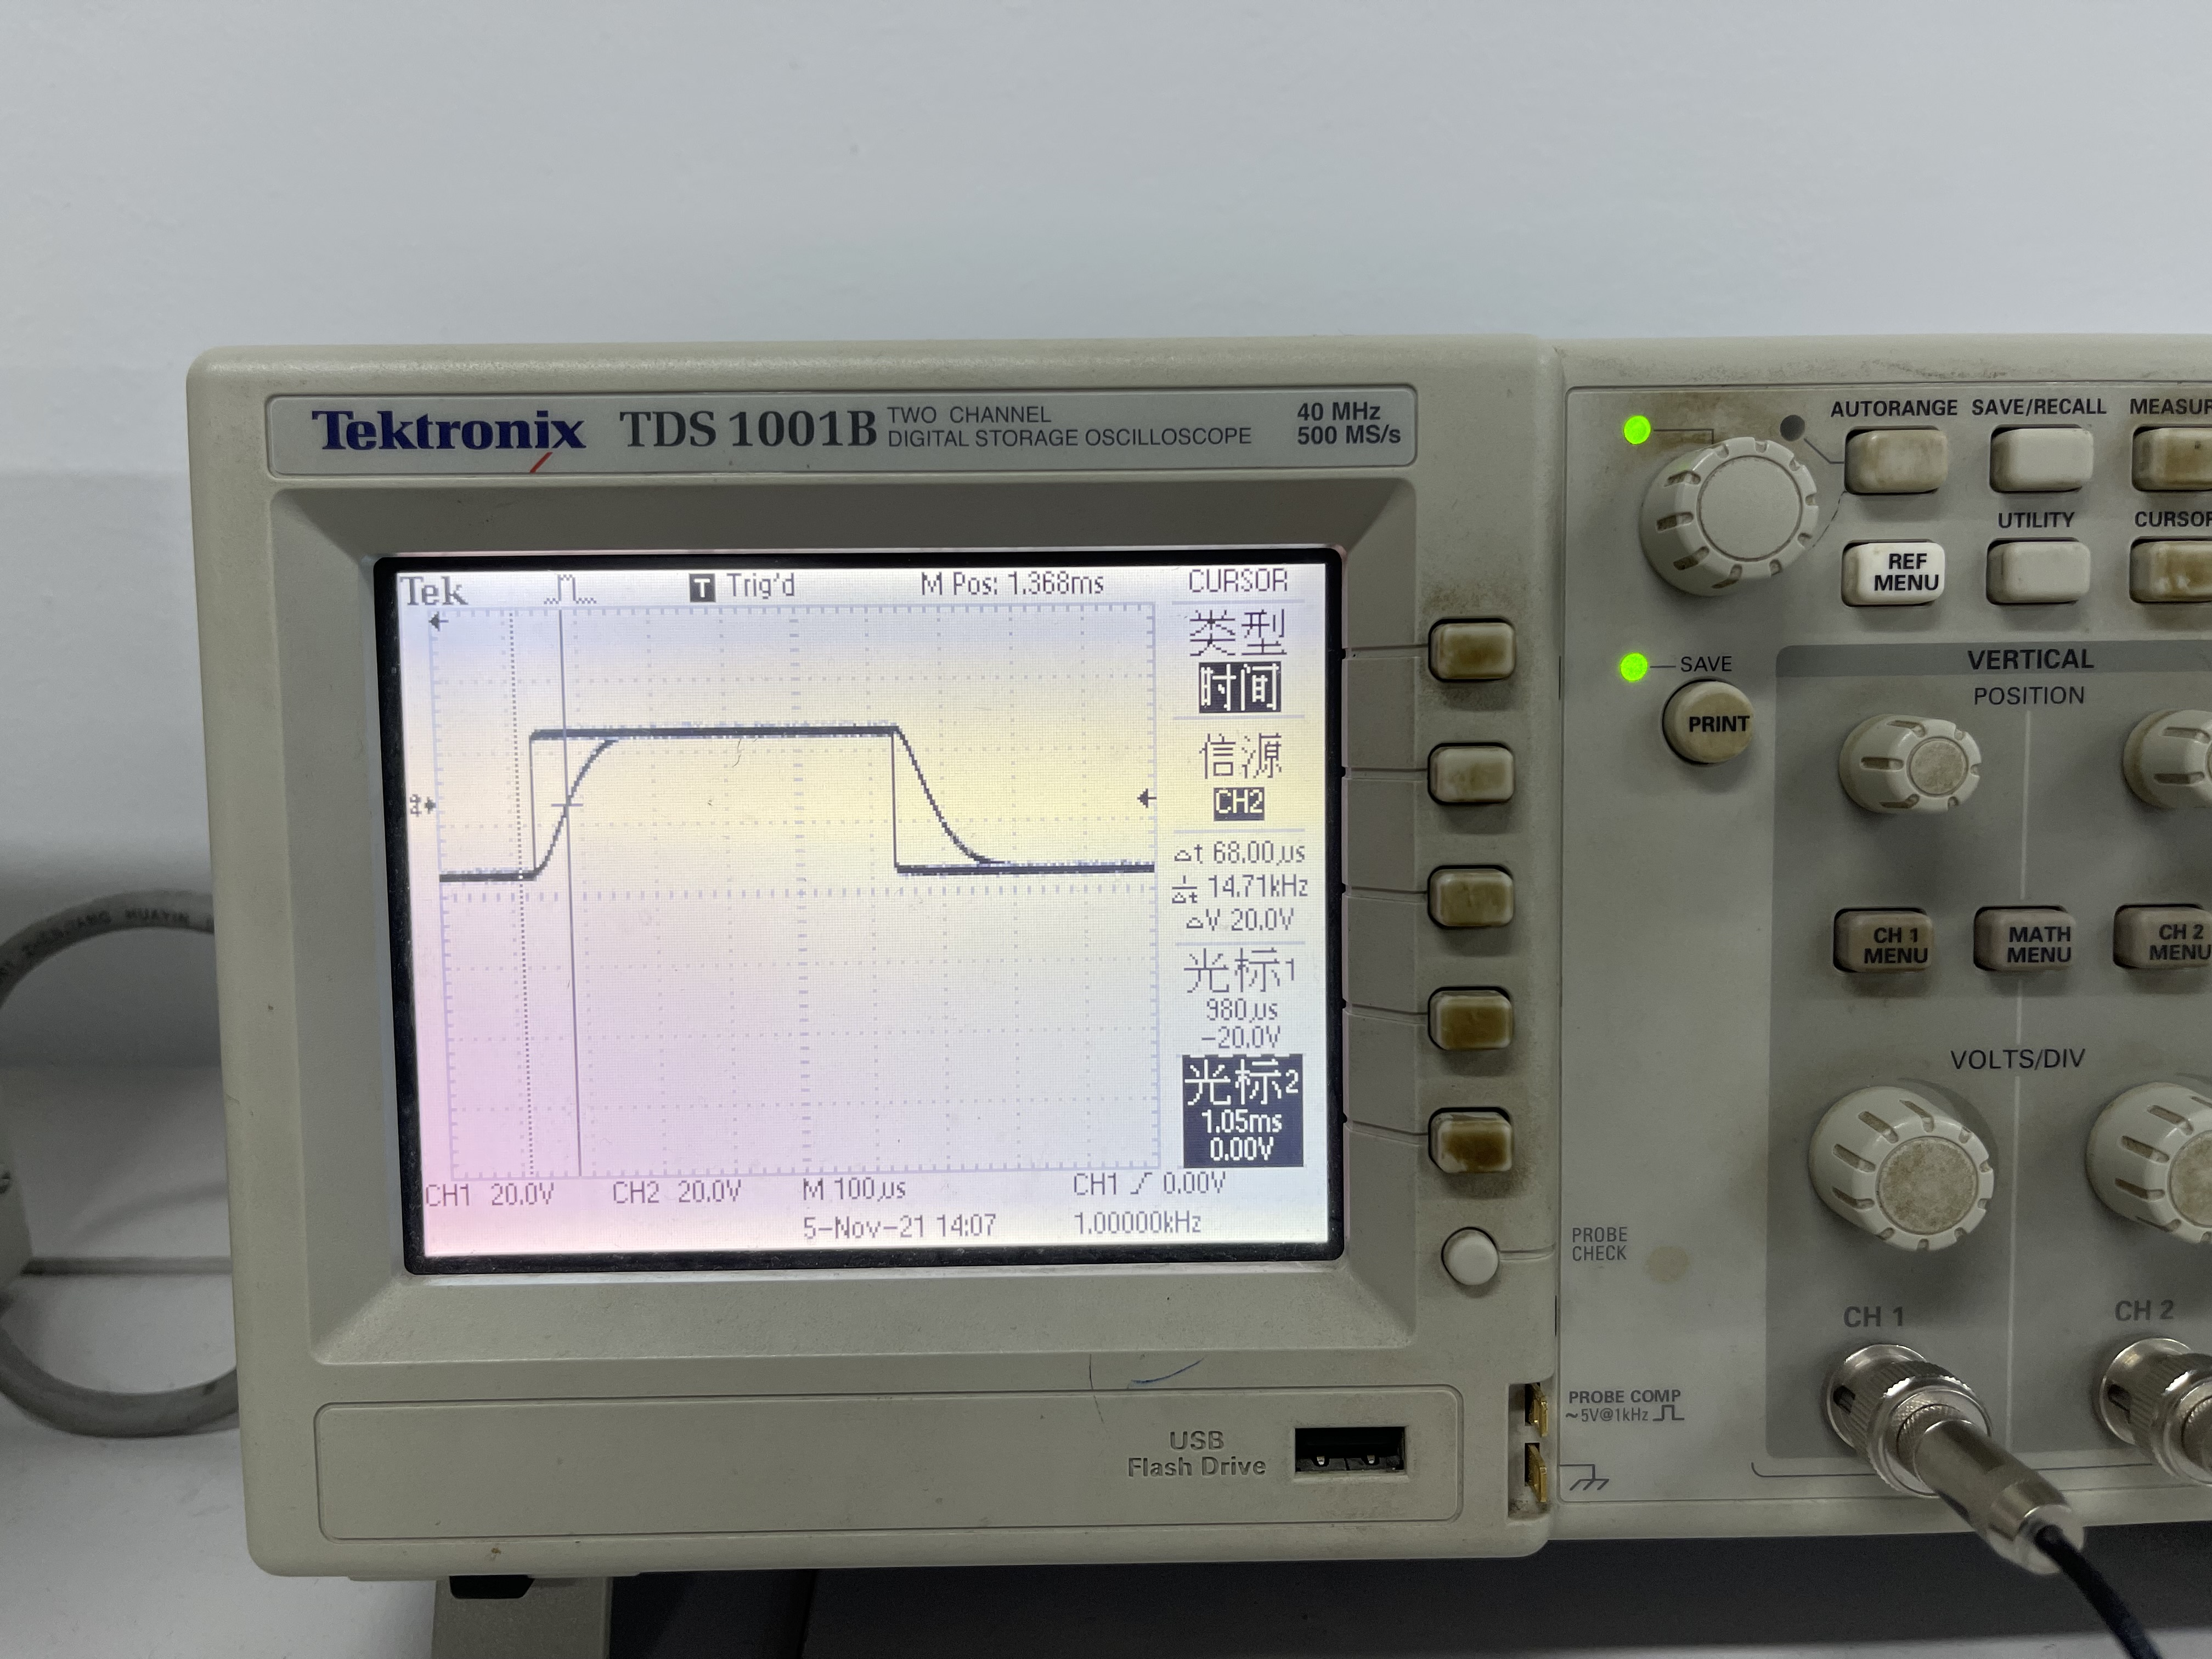
\includegraphics[scale=0.06]{IMG_1830.jpg}
	\caption{RL circuit measurement image}
\end{figure}
\subsection{RLC Series Circuit}
The measurement data of RLC series circuit is shown in the table below:
\begin{table}[H]
	\begin{center}
	\begin{tabular}{|c|c|}
	\hline
	$L$ [$H$] $\pm$ 0 [$H$]	&	0.01	\\
	\hline
	$f$ [$Hz$] $\pm$ 0.001 [$Hz$]	&	1000	\\
	\hline
	$\varepsilon$ [$Vpp$] $\pm$ 0.001 [$Vpp$]	&	4.000	\\
	\hline
	$C$ [$nF$] $\pm$ 0.01 [$nF$]	&	99.88	\\
	\hline
	$T_{0.264}$ [$\mu s$] $\pm$ 0.01 [$\mu s$]	&	32.00	\\
	\hline
	\end{tabular}
	\caption{$T_{0.264}$ measurement data for a critically damped RLC series circuit.}
	\label{tab-3}
	\end{center}
\end{table}

Then we can have:
$$\tau_{theorem} = \frac{1}{\beta} = \sqrt{LC} = 31.622\pm0.01\mu s$$

Compared to the experiment data:
$$\tau_{experiment}=T_{0.264} = 32.00\pm0.0016\mu s$$

The images printed in this experiment are:
\begin{figure}[H]
	\centering
	\subfigure[Underdamped]{ 
	  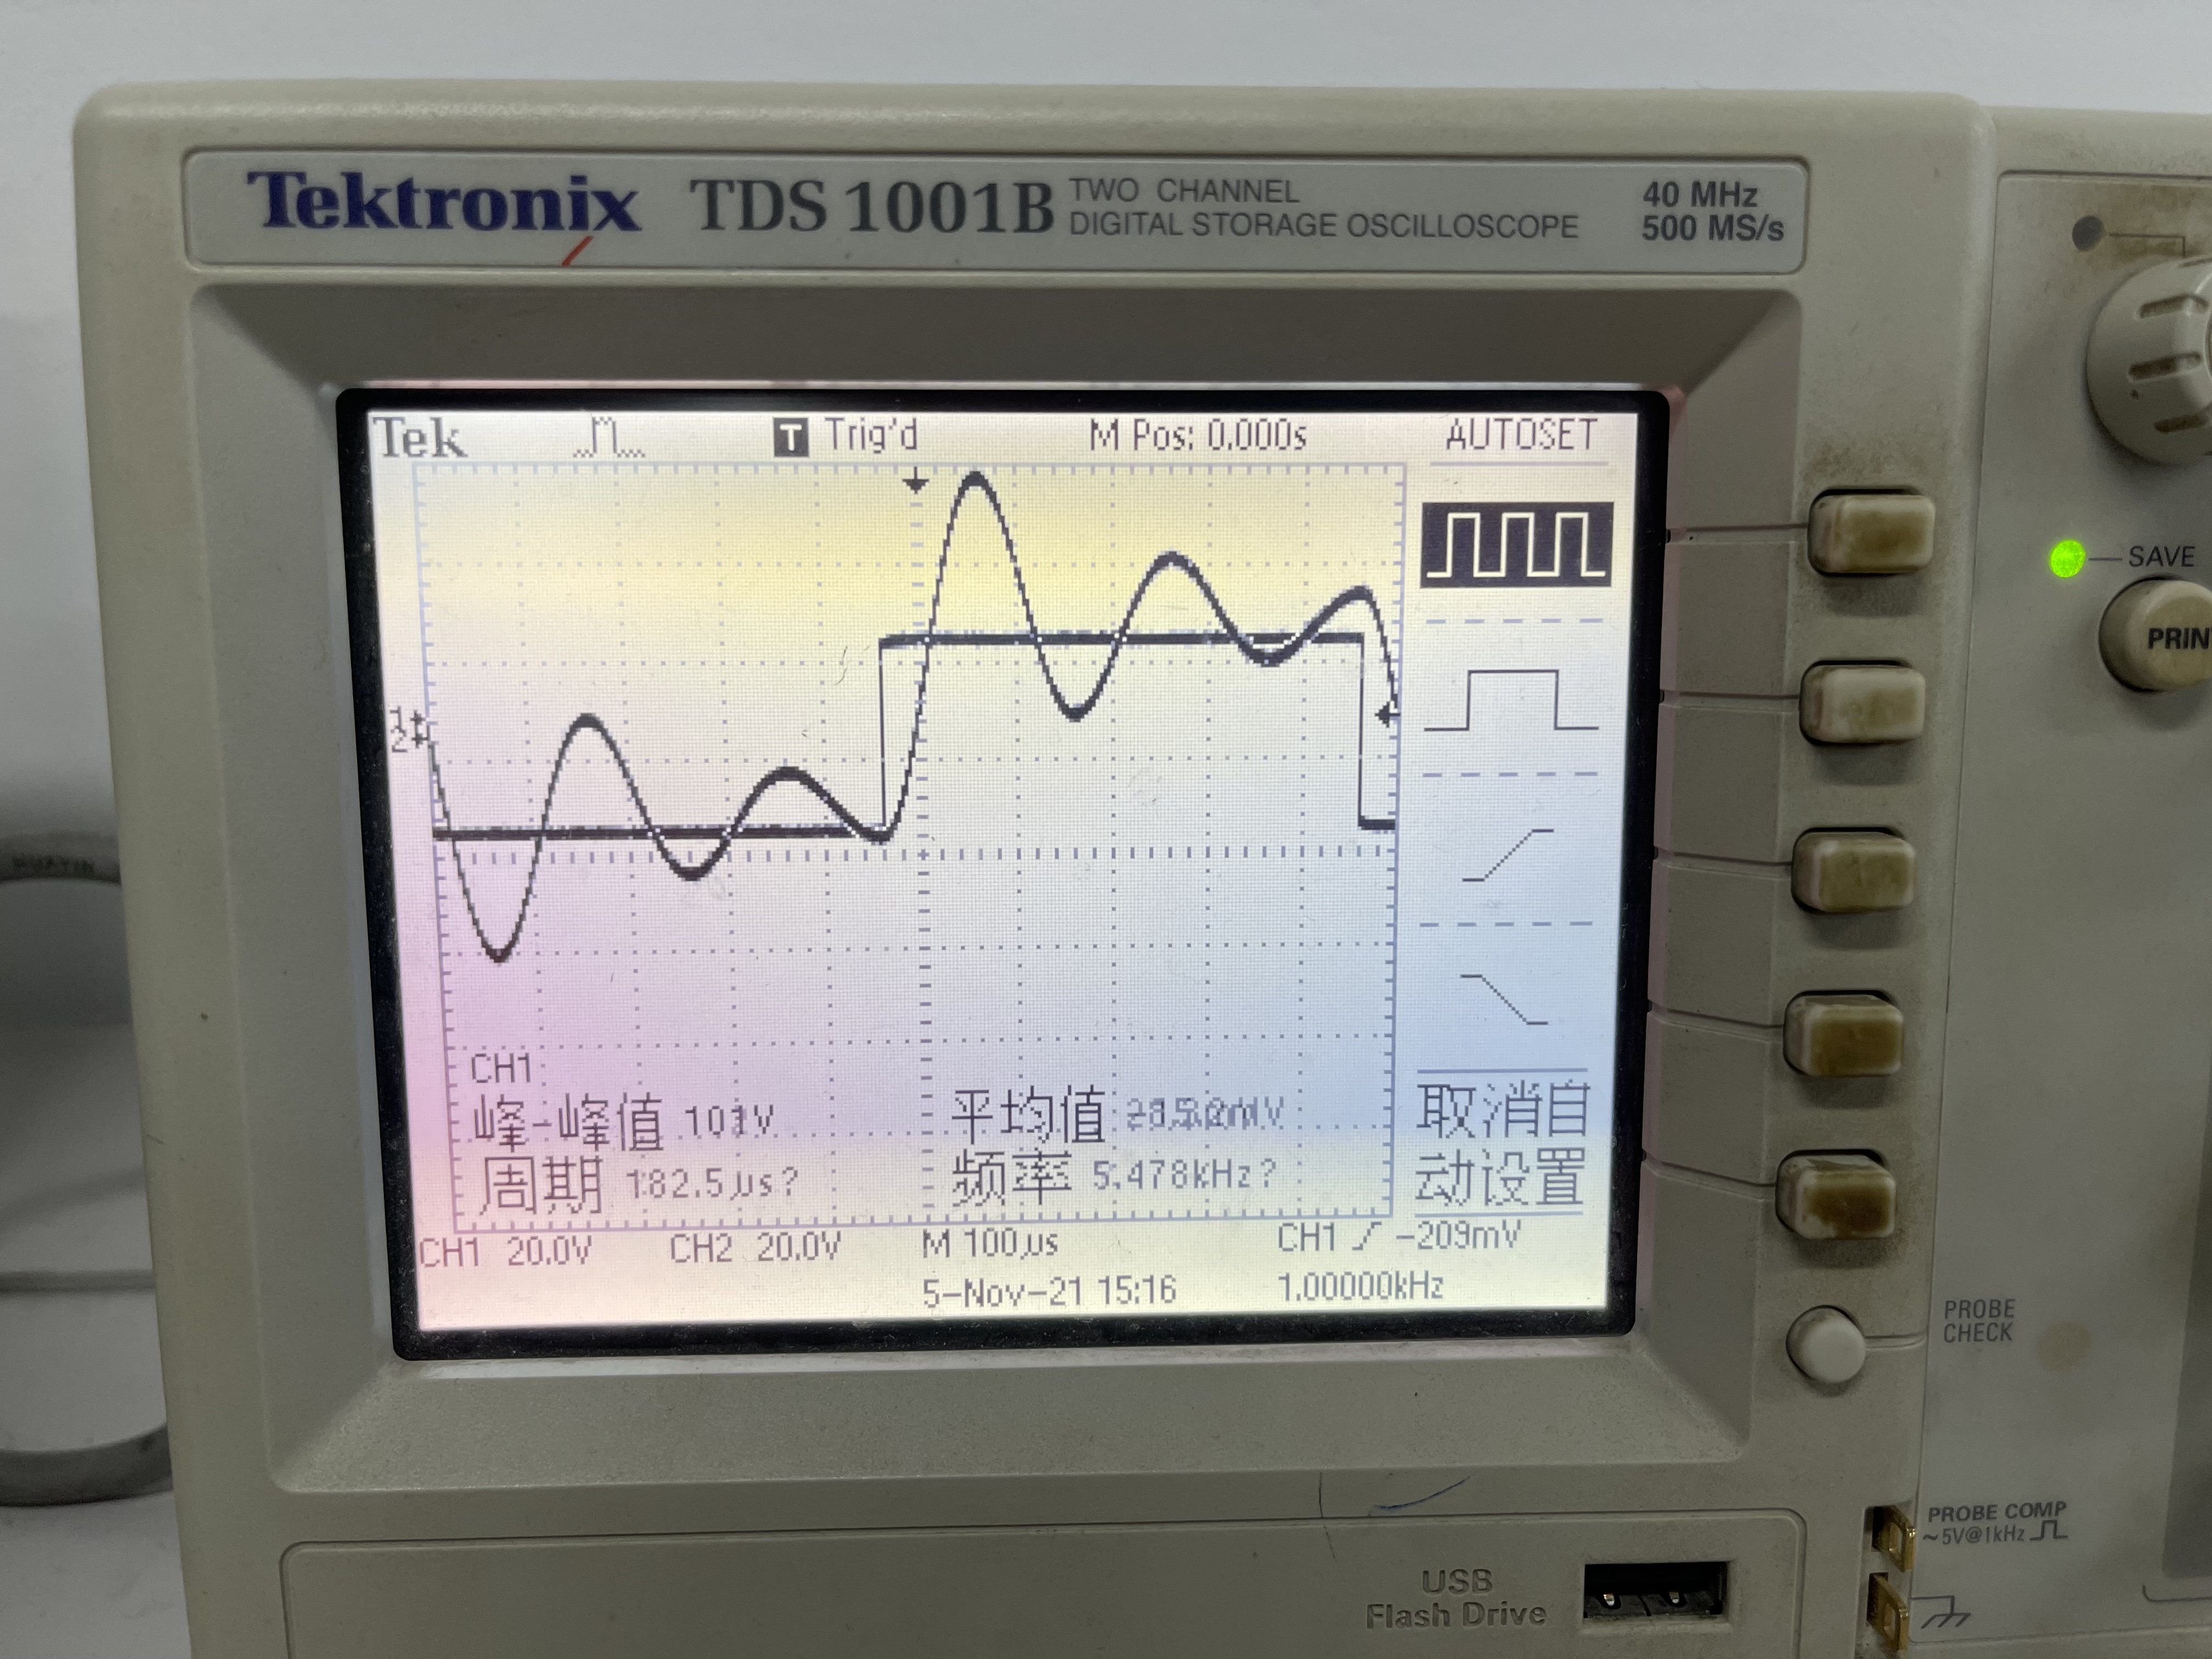
\includegraphics[width=1.5in]{IMG_1834.JPG}} 
	\hspace{0.3in} 
	\subfigure[Critical Damped]{ 
	  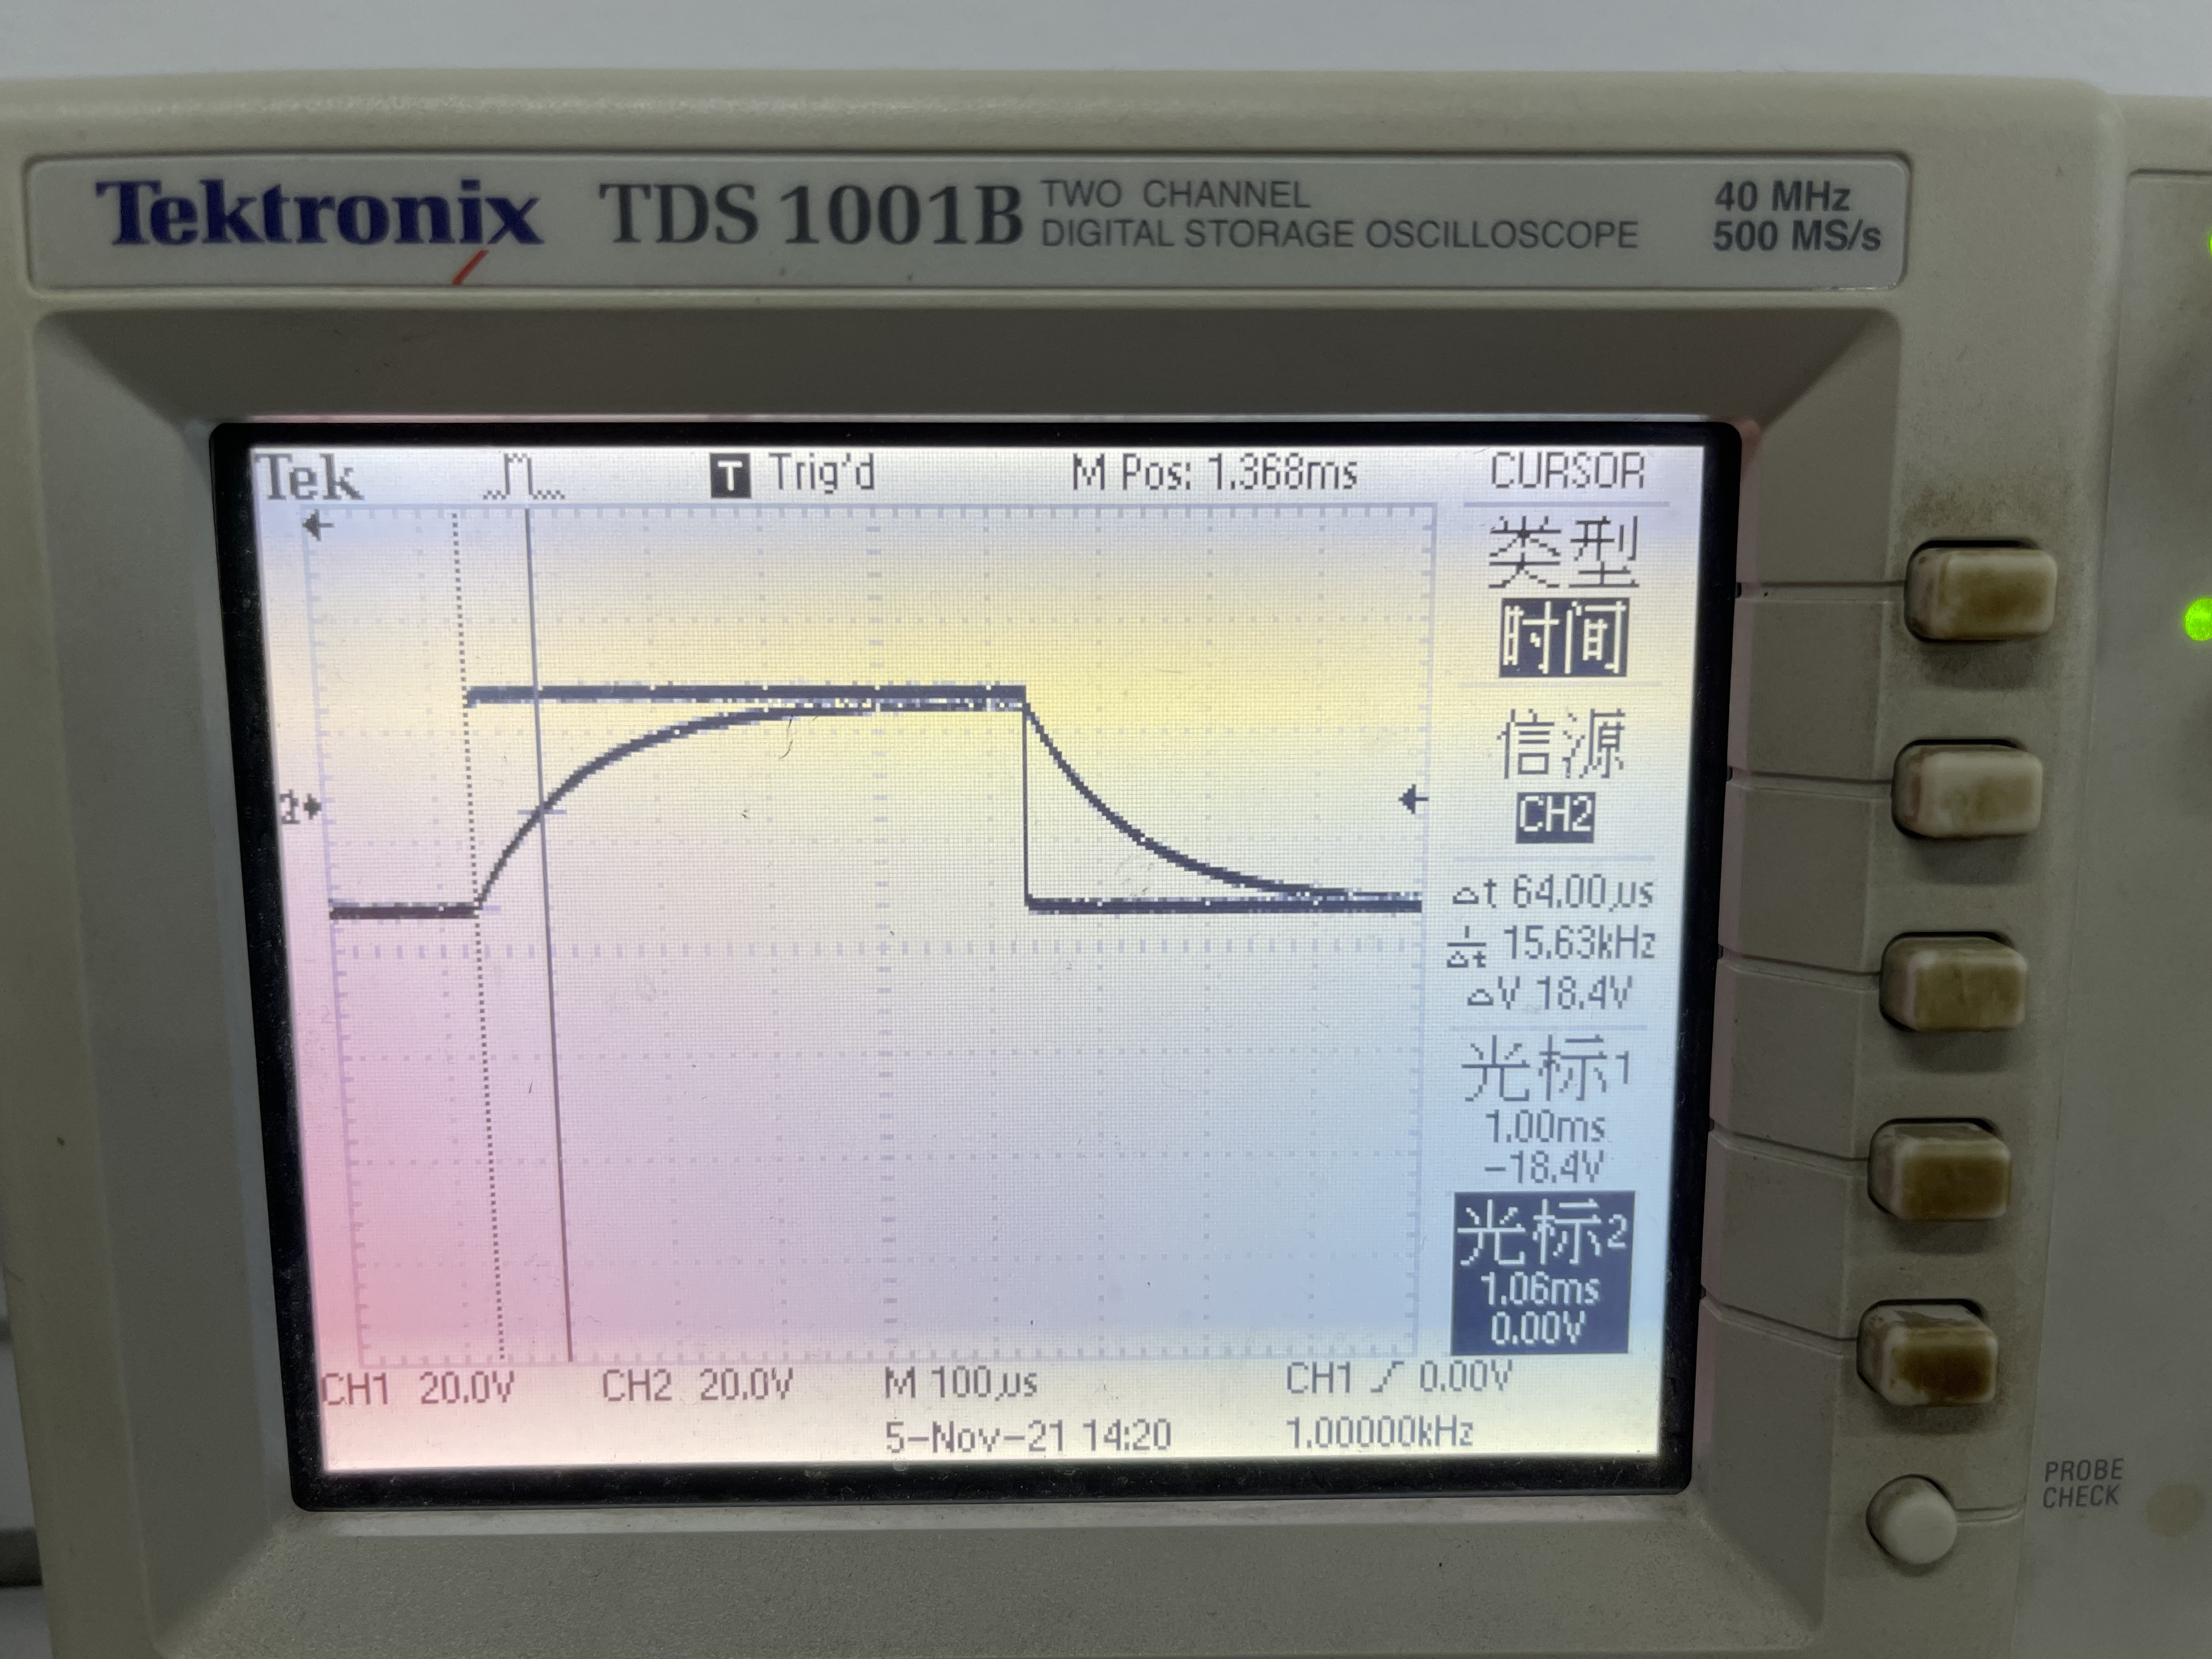
\includegraphics[width=1.5in]{IMG_1833.JPG}} 
	\hspace{0.3in}   
	\subfigure[Overdamped]{ 
	  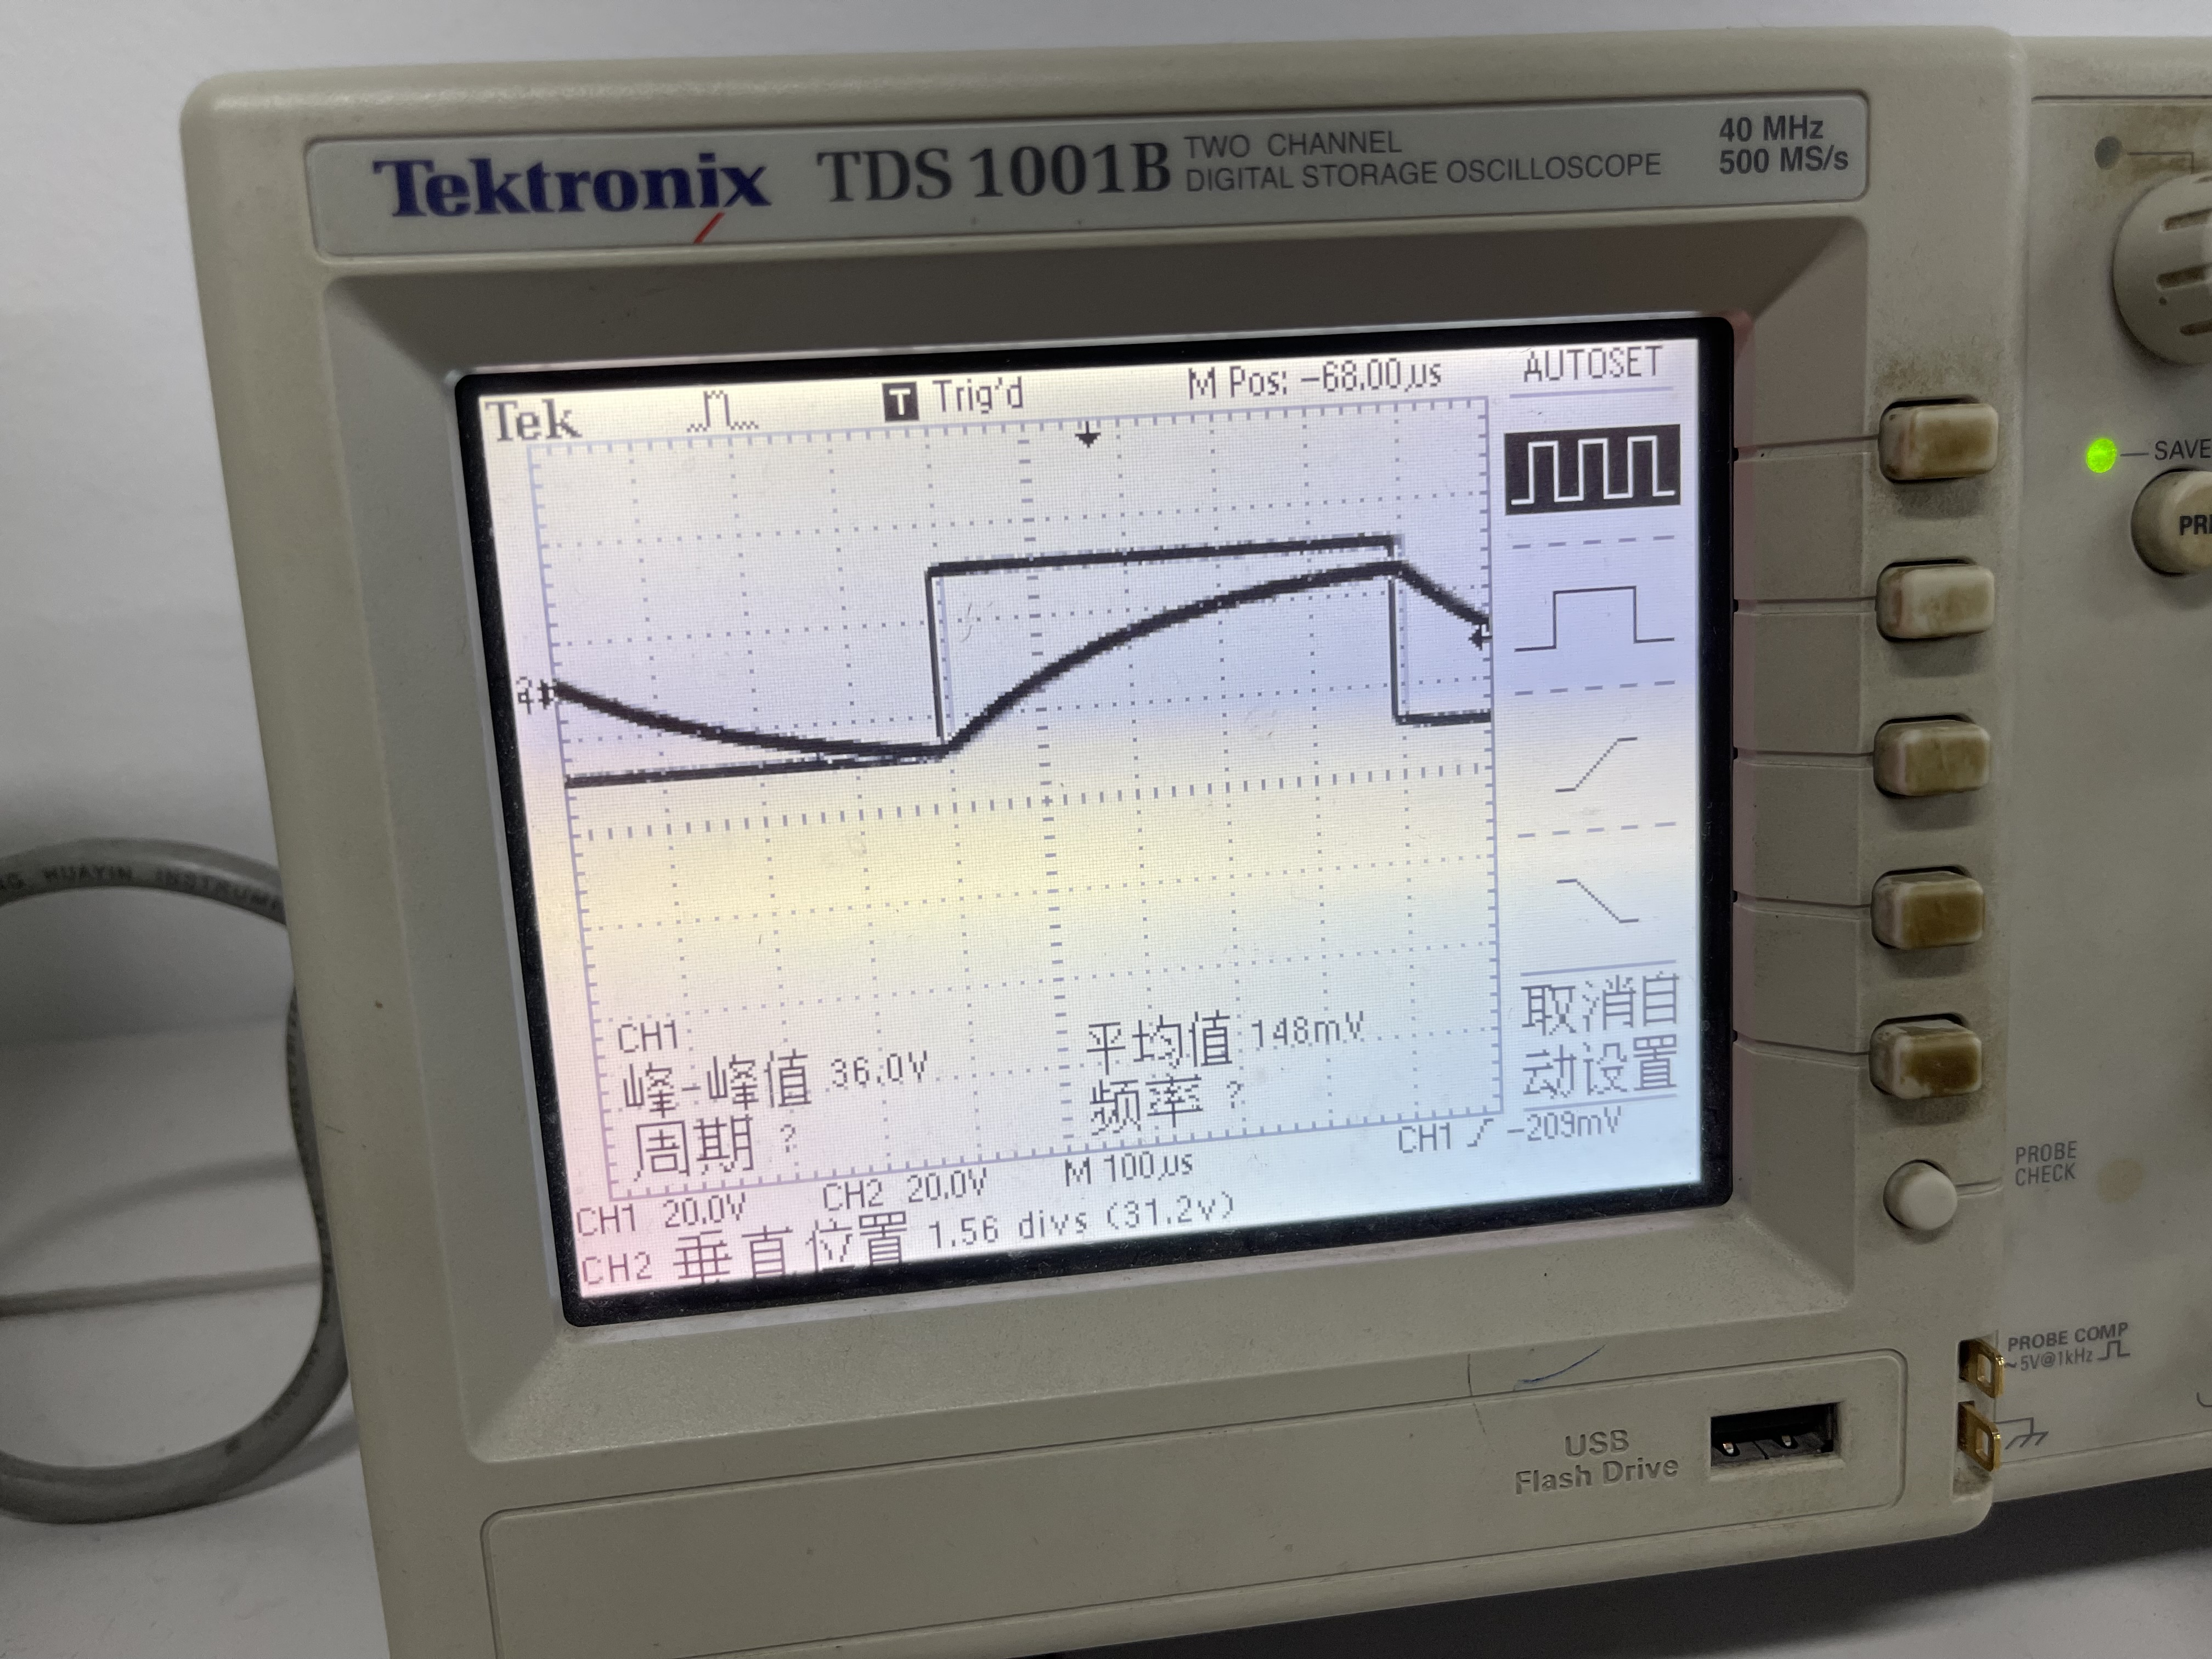
\includegraphics[width=1.5in]{IMG_1835.JPG}} 
	\caption{RLC circuit.}
  \end{figure}
  
\subsection{RLC Resonant Circuit}
The experiment results and uncertainties will be included in Uncertainty section.

The two graphs are plotted by Matlab and are shown below:
\begin{figure}[H]
	\centering
	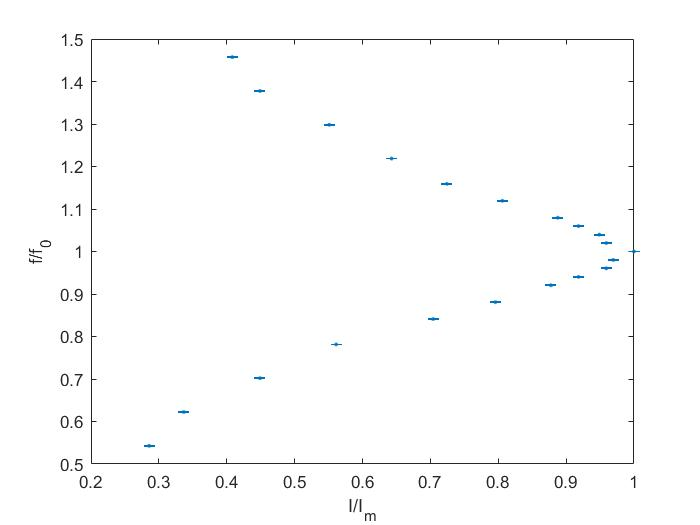
\includegraphics[scale = 0.4]{I_I0vsf_f0.jpg}
	\caption{$I/I_0$ vs. $f/f_0$}
\end{figure}

\begin{figure}[H]
	\centering
	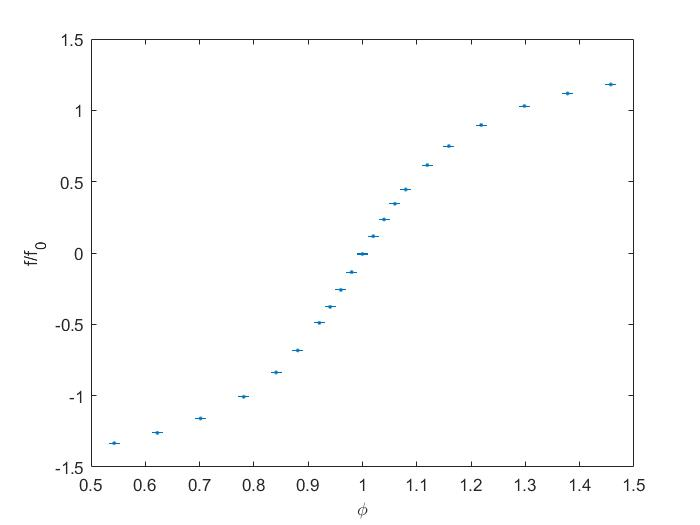
\includegraphics[scale = 0.4]{f_f0vsphi.jpg}
	\caption{$\phi$ vs. $f/f_0$}
\end{figure}

Some of the critical datas are:
$$f_0=5030\,\rm{Hz}$$
$$Q=\frac{\omega_0L}{R}=3.13\pm0.00$$

\section{Uncertainty analysis}
\subsection{Theorem value of $\tau$}
\subsubsection{RC series circuit}
Since the theorem value of $\tau$ in a RC series circuit is calculated from the equation:
$$\tau = RC$$

Then the Uncertainty $u_{\tau}$ can be calculated by the following formula:
\begin{align*}
	u_{\tau}&=\sqrt{\left(\frac{\partial \tau}{\partial R}\right)^2u_R^2+\left(\frac{\partial \tau}{\partial C}\right)^2u_C^2}\\
	&=\sqrt{C^2u_R^2+R^2u_C^2}\\
	&=\sqrt{(99.88nF)^2 \cdot (0.01\Omega)^2 + (99.94\Omega)^2 \cdot (0.01 nF)^2} \\
	&=1.41\times10^{-3}\,\rm{\mu s}
\end{align*}

\subsubsection{RL series circuit}
Since the theorem value of $\tau$ in a RC series circuit is calculated from the equation:
$$\tau = \frac{L}{R}$$

Then the Uncertainty $u_{\tau}$ can be calculated by the following formula:
\begin{align*}
	u_{\tau}&=\sqrt{\left(\frac{\partial \tau}{\partial L}\right)^2u_L^2+\left(\frac{\partial \tau}{\partial R}\right)^2u_R^2}\\
	&=\sqrt{\left(\frac{1}{R}\right)^2u_L^2+\left(\frac{L}{R^2}\right)^2u_R^2}\\
	&=\sqrt{(\frac{1}{99.94\Omega})^2\cdot 0^2 + (\frac{0.01H}{99.94\Omega^2})^2\cdot 0.01\Omega^2}  \\
	&=1.001\times10^{-2}\,\rm{\mu s}
\end{align*}

\subsubsection{RLC Series Circuit}
Since the theorem value of $\tau$ in a RC series circuit is calculated from the equation:
$$\tau = \sqrt{LC}$$

Then the Uncertainty $u_{\tau}$ can be calculated by the following formula:
\begin{align*}
	u_{\tau}&=\sqrt{\left(\frac{\partial \tau}{\partial L}\right)^2u_L^2+\left(\frac{\partial \tau}{\partial C}\right)^2u_C^2}\\
	&=\sqrt{\left(\sqrt{\frac{C}{4L}}\right)^2u_L^2+\left(\sqrt{\frac{L}{4C}}\right)^2u_C^2}\\
	&=\sqrt{(\sqrt{\frac{99.88nF}{4\cdot 0.01H}})^2\cdot 0^2 + (\sqrt{\frac{0.01H}{4\cdot 99.88nF}})^2\cdot (0.01nF)^2}\\
	&=1.582\times10^{-3}\,\rm{\mu s}
\end{align*}

\subsection{Experimental value of $\tau$}
The uncertainty of experimental value of $\tau$ can be calculated by:

$$u_{\tau} \text{ in a RC circuit is } 0.001/\ln2=0.0014\,\rm{\mu s}$$

$$u_{\tau} \text{ in a RL circuit is } 0.01/\ln2=0.014\,\rm{\mu s}$$

$$u_{\tau} \text{ in a RLC circuit is } 0.01/1=0.01\,\rm{\mu s}$$

\subsection{Uncertainty of $f/f_0$ and $I/I_m$}
The uncertainty of $f/f_0$ can be derieved as:
\begin{align*}
	u\left(\frac{f}{f_0}\right) &= \sqrt{\left(\frac{\partial(\frac{f}{f_0})}{\partial f}\right)^2\cdot u_f^2 + \left(\frac{\partial(\frac{f}{f_0})}{\partial f_0}\right)^2\cdot u_{f0}^2}\\
								&= \sqrt{\left(\frac{1}{f_0}\right)^2\cdot u_f^2 + \left(\frac{f}{f_0^2}\right)^2\cdot u^2_{f_0}}\\
\end{align*}

When f = 2730 Hz, the uncertainty of $f/f_0$ is:
\begin{align*}
	u\left(\frac{f}{f_0}\right) &= \sqrt{(1/5030)^2 \cdot 0.001^2 + (2730/5030^2)^2 \cdot 0.001^2}\\
								&= 2.26 \times 10^{-7}\\
\end{align*}

The table of all $u_{f/f_0}$ is shown below:
\begin{table}[H]
	\centering
	\begin{tabular}{|l|l|}
	\hline
	$f/f_0$    & $u_{f/f_0}$ \\ \hline
	0.5427435 & 0.0000002     \\ \hline
	0.6222664 & 0.0000002     \\ \hline
	0.7017893 & 0.0000002     \\ \hline
	0.7813121 & 0.0000003     \\ \hline
	0.8409543 & 0.0000003     \\ \hline
	0.8807157 & 0.0000003     \\ \hline
	0.9204771 & 0.0000003     \\ \hline
	0.9403579 & 0.0000003     \\ \hline
	0.9602386 & 0.0000003     \\ \hline
	0.9801193 & 0.0000003     \\ \hline
	1.0000000 & 0.0000003     \\ \hline
	1.0198807 & 0.0000003     \\ \hline
	1.0397614 & 0.0000003     \\ \hline
	1.0596421 & 0.0000003     \\ \hline
	1.0795229 & 0.0000003     \\ \hline
	1.1192843 & 0.0000003     \\ \hline
	1.1590457 & 0.0000003     \\ \hline
	1.2186879 & 0.0000003     \\ \hline
	1.2982107 & 0.0000003     \\ \hline
	1.3777336 & 0.0000003     \\ \hline
	1.4572565 & 0.0000004     \\ \hline
	\end{tabular}
	\caption{uncertainties of $u_{f/f_0}$}
\end{table}

The uncertainty of $I/Im$ can be derieved as:
\begin{align*}
	u\left(\frac{I}{I_m}\right) &= \sqrt{\left(\frac{\partial(\frac{I}{I_m})}{\partial I}\right)^2\cdot U_I^2 + \left(\frac{\partial(\frac{I}{I_m})}{\partial I_m}\right)^2\cdot U_{I_m}^2}\\
								&= \sqrt{\left(\frac{1}{I_m}\right)^2\cdot U_I^2 + \left(\frac{I}{I_m^2}\right)^2\cdot U^2_{I_m}}\\
\end{align*}

When $U = 1.12$ and $I = U_R/R = 0.011$, the uncertainty of $I/I_m$ is:
\begin{align*}
	u\left(\frac{I}{I_m}\right) &= \sqrt{\left(\frac{1}{0.0392}\right)^2 \cdot (2 \times 10^{-4})^2 + (\frac{0.011}{0.0392^2})^2 \cdot(2\times10^{-4})^2}\\
								&= 0.005\\
\end{align*}
The table of all $u_{I/I_0}$ is shown below:
\begin{table}[H]
	\centering
	\begin{tabular}{|l|l|}
	\hline
	$I/I_0$ & $u_{I/I_0}$ \\ \hline
	0.286   & 0.0053      \\ \hline
	0.337   & 0.0054      \\ \hline
	0.449   & 0.0056      \\ \hline
	0.561   & 0.0058      \\ \hline
	0.704   & 0.0062      \\ \hline
	0.796   & 0.0065      \\ \hline
	0.878   & 0.0068      \\ \hline
	0.918   & 0.0069      \\ \hline
	0.959   & 0.0071      \\ \hline
	0.969   & 0.0071      \\ \hline
	1.000   & 0.0072      \\ \hline
	0.959   & 0.0071      \\ \hline
	0.949   & 0.0070      \\ \hline
	0.918   & 0.0069      \\ \hline
	0.888   & 0.0068      \\ \hline
	0.806   & 0.0066      \\ \hline
	0.724   & 0.0063      \\ \hline
	0.643   & 0.0061      \\ \hline
	0.551   & 0.0058      \\ \hline
	0.449   & 0.0056      \\ \hline
	0.408   & 0.0055      \\ \hline
	\end{tabular}
	\caption{uncertainties of $I/I_0$}
\end{table}



\subsection{The phase $\Phi$}
The phase $\phi$ in a RLC resonant circuit can be calculated by the equation $\phi=tan^{-1}\left(\dfrac{\omega L-\frac{1}{\omega C}}{R}\right)$. Therefore its uncertainty $u_{\phi}$ is found by applying the uncertainty propagation formula

\begin{align*}
	u_{\phi}&=\sqrt{\left(\frac{\partial \phi}{\partial L}\right)^2u_L^2+\left(\frac{\partial \phi}{\partial C}\right)^2u_C^2+\left(\frac{\partial \phi}{\partial R}\right)^2u_R^2+\left(\frac{\partial \phi}{\partial \omega}\right)^2u_\omega^2}\\
	&=\frac{1}{1+\left(\frac{\omega L-\frac{1}{\omega C}}{R}\right)^2}\sqrt{\left(\frac{\omega}{R}\right)^2u_L^2+\left(\frac{1}{\omega RC^2}\right)^2u_C^2+\left(\frac{\omega L-\frac{1}{\omega C}}{R^2}\right)^2u_R^2+\left(\frac{L}{R}-\frac{1}{\omega^2RC}\right)^2u_\omega^2}
\end{align*}

The measurement results and the uncertainties data are shown in the following table:
\begin{table}[H]
	\centering
	\begin{tabular}{|c|c|c|c|}
	\hline
	\multicolumn{2}{|c|}{$R$ [$\Omega$] $\pm$ 0.01 [$\Omega$]}	&	\multicolumn{2}{|c|}{99.94}	\\
	\hline
	\multicolumn{2}{|c|}{$L$ [$H$] $\pm$ 0 [$H$]}	&	\multicolumn{2}{|c|}{0.01}	\\
	\hline
	\multicolumn{2}{|c|}{$C$ [$nF$] $\pm$ 0.01 [$nF$]}	&	\multicolumn{2}{|c|}{99.88}	\\
	\hline
	\multicolumn{2}{|c|}{$f_0$ [$Hz$] $\pm$ 0.001 [$Hz$]}	&	\multicolumn{2}{|c|}{5030}	\\
	\hline
	\multicolumn{2}{|c|}{$\varepsilon$ [$Vpp$] $\pm$ 0.001 [$Vpp$]}	&	\multicolumn{2}{|c|}{4.000}	\\
	\hline
	& $U_R$ [$V$] $\pm$ 0.001 [$V$] & $f$ [$Hz$] $\pm$ 0.001 [$Hz$] & $\phi$ [$rad$]\\
	\hline
	1  & 1.12 & 2730 & -1.333$\pm$0.000 \\ \hline
	2  & 1.32 & 3130 & -1.261$\pm$0.000 \\ \hline
	3  & 1.76 & 3530 & -1.160$\pm$0.000 \\ \hline
	4  & 2.20 & 3930 & -1.008$\pm$0.000 \\ \hline
	5  & 2.76 & 4230 & -0.837$\pm$0.000 \\ \hline
	6  & 3.12 & 4430 & -0.683$\pm$0.000 \\ \hline
	7  & 3.44 & 4630 & -0.490$\pm$0.000 \\ \hline
	8  & 3.60 & 4730 & -0.378$\pm$0.000 \\ \hline
	9  & 3.76 & 4830 & -0.259$\pm$0.000 \\ \hline
	10 & 3.80 & 4930 & -0.134$\pm$0.000 \\ \hline
	11 & 3.92 & 5030 & -0.007$\pm$0.000 \\ \hline
	12 & 3.76 & 5130 & 0.117$\pm$0.000  \\ \hline
	13 & 3.72 & 5230 & 0.235$\pm$0.000  \\ \hline
	14 & 3.60 & 5330 & 0.345$\pm$0.000  \\ \hline
	15 & 3.48 & 5430 & 0.445$\pm$0.000  \\ \hline
	16 & 3.16 & 5630 & 0.616$\pm$0.000  \\ \hline
	17 & 2.84 & 5830 & 0.749$\pm$0.000  \\ \hline
	18 & 2.52 & 6130 & 0.897$\pm$0.000  \\ \hline
	19 & 2.16 & 6530 & 1.030$\pm$0.000  \\ \hline
	20 & 1.76 & 6930 & 1.118$\pm$0.000  \\ \hline
	21 & 1.60 & 7330 & 1.181$\pm$0.000  \\ \hline
	\end{tabular}
	\caption{Measurement data for the $U_R$ vs. $f$ dependence for a RLC resonant circuit.}
	\label{tab-4}
	\end{table}



\subsection{The quality factor Q}
The theorem value of $Q$ in a RL series circuit can be calculated by the equation $Q=\frac{\omega_0 L}{R}$. Therefore its uncertainty $u_Q$ is found by applying the uncertainty propagation formula
\begin{align*}
	u_{Q}&=\sqrt{\left(\frac{\partial Q}{\partial \omega_0}\right)^2u_{\omega_0}^2+\left(\frac{\partial Q}{\partial L}\right)^2u_L^2+\left(\frac{\partial Q}{\partial R}\right)^2u_R^2}\\
	&=\sqrt{\left(\frac{L}{R}\right)^2u_{\omega_0}^2+\left(\frac{\omega_0}{R}\right)^2u_L^2+\left(\frac{\omega_0L}{R^2}\right)^2u_R^2}\\
	&=3.28\times10^{-4}
\end{align*}

\section{Conclusion and discussion}
\subsection{Conclusions}
In this experiment, we understand the physics of alternating-current circuits, 
in particular the processes of charging/discharging of capacitors, the phenomenon 
of electromagnetic induction in inductive elements, and other dynamic processes in RC, 
RL, and RLC series circuits. Moreover, methods for measuring the amplitude-frequency and 
the phase-frequency characteristics of RC, RL, and RLC series circuits will be studied. 
The resonance frequency of a RLC circuit as well as the quality factor of the circuit will
 be found from the amplitude-frequency curve.

In a RC series circuit, we obsered the waveshape of $U_C$ in the charging and discharging part. 
The wave shape is a exponential wave, and the time constant can be derived as: 
$$\tau=RC$$
The measuerd data is quite different from the theoretical data, and the reason will be discussed at 
the end of this section.

In a RL series circuit, we can also observe that the wave is a exponential wave, which has a 
similar equation to that of RC series circuit. The time constant can be derieved as:
$$\tau=\frac{L}{R}$$
The relative error between the experiment data and theoretical data is $0.24\%$, which is relatively 
small and can prove the experiment and formula valid.

For a RLC series circuit, the waveform is a oscillation damped wave, and the damped type depends on 
the resistor, condutor and inductor chosen. When the RLC series circuit is critically damped, we can find:
$$\tau=\sqrt{LC}$$

Then we discovered the RLC resonant circuit, which is similar to a simple harmonic 
oscillation. We plotted the experiment results in certain method so that we can find the 
property of it. We also calculated the The quality factor $Q$ within the theorem.
\\
\subsection{Discussions}
In RC sries circuit experiment, the experiment data is very different from the theorum data. 
This is because I falsely set the start place of the cursor, and measured the wrong time period.

In RC, RL, RLC series circuits experiments, the measurements of $T_{1/2}$ and $T_{0.264}$ might be 
inaccurate, because it's hard to locate the cursor on exactly the peak of the graph with human eyes only. If only the 
oscillator can read the y-value of the wave, we can read the height and observe whether it has changed 
or not. At the exact point the y-value starts to decrease is the point we want to start measurement.



\section{References}
    \begin{enumerate}
        \item Qin Tian, Cao Jianjun, Yi Hankun, Wu Ziyou, Zhang Yifei, Yao Yuan, Mateusz Krzyzosiak
    \end{enumerate}

\end{document}
